% lint-skip: 未完成ステータス（figure/table caption 未対応，人手チェック時に解消予定）
\documentclass[../../main.tex]{subfiles}
\begin{document}

\begin{flushright}
  \footnotesize\textit{【自動文字起こし・要確認】}
\end{flushright}

［解1］座標平面で，$A(0, a)$, $B(b, 0)$, $C(c, 0)$ ($a>0, b>0, c<0$) として良い．$PQ$ の中点の軌跡を考える．まず，$P, Q$ が $AC, BC$ 上を動く時，
\[
  P(ct, a(1-t)), \quad Q(s, 0) \quad (0 \le t \le 1, c \le s \le b)
\]
とおける．$PQ$ の中点 $R(X, Y)$ とすると
\[
  \begin{pmatrix} X \\ Y
  \end{pmatrix} = \dfrac{1}{2}
  \begin{pmatrix} ct \\ a(1-t)
  \end{pmatrix} + \dfrac{1}{2}
  \begin{pmatrix} s \\ 0
  \end{pmatrix} = \dfrac{1}{2} t
  \begin{pmatrix} c \\ -a
  \end{pmatrix} + \dfrac{1}{2} s
  \begin{pmatrix} 1 \\ 0
  \end{pmatrix} + \dfrac{1}{2}
  \begin{pmatrix} 0 \\ a
  \end{pmatrix}
\]
だから，$R$ の軌跡は後掲の図の色付き部分のようである（境界含む）．

\begin{figure}[htb]
  \centering
  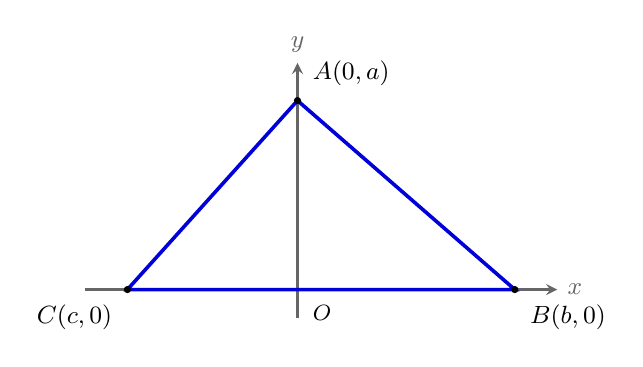
\begin{tikzpicture}[x=1.2cm, y=1.2cm, >=stealth, every node/.style={font=\small}]
    \coordinate (A) at (0, 2);
    \coordinate (B) at (2.3, 0);
    \coordinate (C) at (-1.8, 0);
    \draw[->, thick, gray!80!black] (-2.25, 0) -- (2.75, 0) node[right] {$x$};
    \draw[->, thick, gray!80!black] (0, -0.3) -- (0, 2.4) node[above] {$y$};
    \draw[line width=1.3pt, blue!85!black] (A) -- (B) -- (C) -- cycle;
    \fill (A) circle (1.3pt) node[above right=2pt] {$A(0,a)$};
    \fill (B) circle (1.3pt) node[below right=2pt] {$B(b,0)$};
    \fill (C) circle (1.3pt) node[below left=2pt] {$C(c,0)$};
    \node[below right=2pt, font=\footnotesize] at (0,0) {$O$};
  \end{tikzpicture}
  \caption{頂点 $A,B,C$ の座標を定めた三角形}
  \label{fig:1962_1_coordinates}
\end{figure}

$PQ$ が
$
\begin{cases} 1^\circ \quad AC, AB \text{ 上の時} \\ 2^\circ \quad AB, BC \text{ 上の時}
\end{cases}$
も，対称性から $R$ の軌跡は以下のようになる（境界含む）．

\begin{figure}[htb]
  \centering
  \begin{tikzpicture}[x=0.84cm, y=0.84cm, >=stealth,
    every node/.style={font=\footnotesize}]
    % Each shaded locus is the Minkowski midpoint set of the two named sides.
    \foreach \dx/\panelname/\kind in
    {0/{AC,BC}/1, 5.2/{AC,AB}/2, 10.4/{AB,BC}/3} {
      \begin{scope}[shift={(\dx,0)}]
        \coordinate (A) at (0, 2);
        \coordinate (B) at (2.3, 0);
        \coordinate (C) at (-1.8, 0);
        \coordinate (ABmid) at ($(A)!0.5!(B)$);
        \coordinate (ACmid) at ($(A)!0.5!(C)$);
        \coordinate (BCmid) at ($(B)!0.5!(C)$);
        \ifnum\kind=1
        \fill[teal!20] (C) -- (ACmid) -- (ABmid) -- (BCmid) -- cycle;
        \else
        \ifnum\kind=2
        \fill[blue!18] (A) -- (ACmid) -- (ABmid) -- cycle;
        \else
        \fill[orange!22] (ACmid) -- (ABmid) -- (B) -- (BCmid) -- cycle;
        \fi
        \fi
        \draw[->, gray!75!black] (-2.1, 0) -- (2.6, 0) node[right] {$x$};
        \draw[->, gray!75!black] (0, -0.25) -- (0, 2.35) node[above] {$y$};
        \draw[thick, blue!85!black] (A) -- (B) -- (C) -- cycle;
        \draw[dashed, gray!70!black] (ACmid) -- (ABmid);
        \node[above=2pt] at (A) {$A$};
        \node[below right=1pt] at (B) {$B$};
        \node[below left=1pt] at (C) {$C$};
        \node[below=13pt, font=\small] at (0.25, 0) {$\panelname$};
      \end{scope}
    }
  \end{tikzpicture}
  \caption{$P,Q$ がそれぞれ異なる辺上を動くときの中点の領域（境界を含む）}
  \label{fig:1962_1_pair_regions}
\end{figure}

以上まとめて，$AB, BC, CA$ の中点を $\alpha, \beta, \gamma$ として，以下のようになる．

\begin{figure}[htb]
  \centering
  \begin{tikzpicture}[x=1.4cm, y=1.4cm, every node/.style={font=\small}]
    \coordinate (A) at (0, 2.5);
    \coordinate (B) at (-2.2, 0);
    \coordinate (C) at (2.2, 0);
    \coordinate (alpha) at ($(A)!0.5!(B)$);
    \coordinate (beta) at ($(B)!0.5!(C)$);
    \coordinate (gamma) at ($(C)!0.5!(A)$);
    \fill[blue!10] (A) -- (alpha) -- (gamma) -- cycle;
    \fill[blue!10] (B) -- (beta) -- (alpha) -- cycle;
    \fill[blue!10] (C) -- (gamma) -- (beta) -- cycle;
    \fill[teal!22] (alpha) -- (beta) -- (gamma) -- cycle;
    \draw[line width=1.3pt, blue!85!black] (A) -- (B) -- (C) -- cycle;
    \draw[thick, dashed, teal!80!black] (alpha) -- (beta) -- (gamma) -- cycle;
    \node[above=2pt] at (A) {$A$};
    \node[below left=2pt] at (B) {$B$};
    \node[below right=2pt] at (C) {$C$};
    \node[left=2pt] at (alpha) {$\alpha$};
    \node[below=2pt] at (beta) {$\beta$};
    \node[right=2pt] at (gamma) {$\gamma$};
    \node at (0, 1.95) {$1$ 本};
    \node at (-1.15, 0.4) {$1$ 本};
    \node at (1.15, 0.4) {$1$ 本};
    \node at (0, 0.84) {$3$ 本};
    \node[fill=white, inner sep=1pt, font=\footnotesize] at (0, 1.25) {$2$ 本};
    \node[fill=white, inner sep=1pt, font=\footnotesize] at (-0.55, 0.62) {$2$ 本};
    \node[fill=white, inner sep=1pt, font=\footnotesize] at (0.55, 0.62) {$2$ 本};
  \end{tikzpicture}
  \caption{三辺の中点 $\alpha,\beta,\gamma$ と通る線分の本数}
  \label{fig:1962_1_counts}
\end{figure}

［解2］（解1の最後の図を用いる）

$\triangle A\alpha\gamma, \triangle B\beta\alpha, \triangle C\gamma\beta$（辺 $\beta\alpha, \gamma\alpha, \gamma\beta$ をのぞく）の周及び内部を $T_1$，

辺 $\beta\alpha, \gamma\alpha, \gamma\beta$ を $T_2$，

$\triangle \alpha\beta\gamma$ の内部を $T_3$

とする．$M$ が各々の領域をうごく時の線本数をしらべる．まず $T_3$ について．

\begin{figure}[htb]
  \centering
  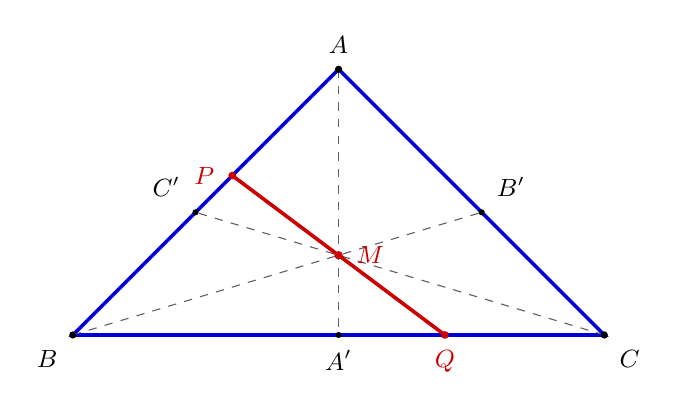
\begin{tikzpicture}[x=1.35cm, y=1.35cm, every node/.style={font=\small}]
    \coordinate (A) at (0, 2.5);
    \coordinate (B) at (-2.5, 0);
    \coordinate (C) at (2.5, 0);
    \coordinate (M) at (0, 0.75);
    \coordinate (Ap) at (0, 0);
    \coordinate (Bp) at (1.346, 1.154);
    \coordinate (Cp) at (-1.346, 1.154);
    \coordinate (P) at (-1, 1.5);
    \coordinate (Q) at (1, 0);
    \draw[line width=1.3pt, blue!85!black] (A) -- (B) -- (C) -- cycle;
    \draw[dashed, gray!75!black] (A) -- (Ap);
    \draw[dashed, gray!75!black] (B) -- (Bp);
    \draw[dashed, gray!75!black] (C) -- (Cp);
    \draw[line width=1.3pt, red!80!black] (P) -- (Q);
    \fill (A) circle (1.3pt) node[above=2pt] {$A$};
    \fill (B) circle (1.3pt) node[below left=2pt] {$B$};
    \fill (C) circle (1.3pt) node[below right=2pt] {$C$};
    \fill (Ap) circle (1.1pt) node[below=2pt] {$A'$};
    \fill (Bp) circle (1.1pt) node[above right=2pt] {$B'$};
    \fill (Cp) circle (1.1pt) node[above left=2pt] {$C'$};
    \fill[red!80!black] (P) circle (1.4pt) node[left=3pt] {$P$};
    \fill[red!80!black] (Q) circle (1.4pt) node[below=2pt] {$Q$};
    \fill[red!80!black] (M) circle (1.5pt) node[right=3pt] {$M$};
  \end{tikzpicture}
  \caption{中央の領域にある $M$ を通る線分 $PQ$ と各頂点から $M$ への直線}
  \label{fig:1962_1_central_segment}
\end{figure}

$AM$ と $BC$，$BM$ と $AC$，$CM$ と $AB$ の交点を各々 $A', B', C'$ とする．$P \in A$ から，$Q$ を $A'$ から，反時計回りに $PQ$ が $M$ を通るようにうごかす．（$P$ は $A \to C' \to B \to A'$，$Q$ は $A' \to C \to B' \to A$）

\[
  |MA| - |MA'| > 0, \quad |MC'| - |MC| < 0
\]
から，$P$ が $A \to C'$ とうごく時，
\[
  |MP| - |MQ|
\]
はレンゾクな値をとりながら正 $\to$ 負と変化するので，$|MP| - |MQ| = 0$ となる $(P, Q)$ の組が少なくとも1つ存在する．このような組が2つ以上あると仮定すると，これらを $(P_1, Q_1), (P_2, Q_2)$ として，この4点は平行四辺形をなすが，$AB \mathbin{/\!/} BC$ 等より矛盾．よって $|MP| - |MQ| = 0$ となる $(P, Q)$ がただ1つ存在する．同様に $P$ が $C' \to B, B \to A'$ と動く時にも1つずつ，計3つある．

同様に $T_2$ のときは2つ，$T_1$ のときは1つあるので，［解1］のようになる．

\newpage

\end{document}
